
\section*{CHƯƠNG 1. GIỚI THIỆU VỀ TỔ CHỨC TIẾP NHẬN}
\setcounter{section}{1}
\setcounter{subsection}{0} %LƯU Ý MỖI LẦN THÊM CHƯƠNG MỚI CẦN THÊM CÂU NÀY ĐỂ RESET THỨ TỰ CỦA SUBSECTON VỀ 1
\setcounter{table}{0} % LƯU Ý SAU MỖI LẦN GỌI BẢNG HAY HÌNH ẢNH PHẢI THÊM CÂU NÀY ĐỂ RESET THỨ TỰ
\setcounter{figure}{0} %% LƯU Ý SAU MỖI LẦN GỌI BẢNG HAY HÌNH ẢNH PHẢI THÊM CÂU NÀY ĐỂ RESET THỨ TỰ
\addcontentsline{toc}{section}{\numberline{}CHƯƠNG 1. GIỚI THIỆU VỀ TỔ CHỨC TIẾP NHẬN}
Trong chương này, em xin phép được trình bày về chức năng, nhiệm vụ, cơ cấu tổ chức của công ty
tiếp nhận thực tập. Cùng với đó là các sản phẩm và các hoạt động mà công ty đang thực hiện 
trong thời gian em thực tập.

\subsection{Giới thiệu tổng quan}
Tổ chức tiếp nhận thực tập em là công ty TNHH Pancake Việt Nam, công ty chuyên cung cấp các giải pháp
hỗ trợ doanh nghiệp quản lý kinh doanh toàn diện với các sản phẩm phần mềm hỗ trợ người dùng bán hàng đa nền
tảng trên mạng xã hội cũng như trên các sàn thương mại điện tử. Các sản phẩm tạo thành một hệ sinh thái hỗ trợ
tối đa cho người dùng về mọi mặt khi muốn kinh doanh online.

\begin{figure}[H]
  \centering
  \includegraphics[width=15cm,height=7cm]{Images/pancake/all_items_pancake.png}
  \caption[Hình ảnh giới thiệu các sản phẩm]{\bfseries \fontsize{12pt}{0pt}blame
  \selectfont Hình ảnh giới thiệu các sản phẩm}
  \label{ttlk} %đặt tên cho ảnh
\end{figure}

\subsubsection{Các sản phẩm của công ty}
\paragraph{Pancake \cite{pancake}}
\mbox{}

Pancake là phần mềm quản lý bán hàng toàn diện trên mạng xã hội và các nền tảng thương mại điện tử. 
\begin{figure}[H]
  \centering
  \includegraphics[width=8cm,height=6cm]{Images/pancake/pancake.png}
  \caption[Hình ảnh giới thiệu Pancake]{\bfseries \fontsize{12pt}{0pt}
  \selectfont Hình ảnh giới thiệu Pancake}
  \label{ttlk} %đặt tên cho ảnh
\end{figure}

Với các tính năng: 
\begin{itemize}
  \item Tính năng cho phép người dùng gộp nhiều pages để quản lý chung ở 1 giao diện
  \item Thống kê chi tiết theo ngày, giờ. Lượng khách hàng mới và tỉ lệ chốt đơn hằng ngày
  \item Cho phép tùy chỉnh cài đặt phân công hội thoại, phân chia việc cho nhân viên
  \item Tạo đơn hàng và gửi hóa đơn trong live chat. Đồng bộ dữ liệu với POS
\end{itemize}
Pancake tích hợp nhiều tính năng đồng hộ cho cho việc quản lý bán hàng từ cửa hàng đến các kênh online. 
Tăng năng suất, giảm chi phí!

\paragraph{Pancake Chat \cite{panchat}}
\mbox{}

Pancake Work là phần mềm chat trao đổi thông tin nội bộ với các chế độ quản lý công việc, 
giúp các nhà quản lý có thể kiểm soát luồng công việc dễ dàng hiệu quả.
\begin{figure}[H]
  \centering
  \includegraphics[width=11cm,height=11cm]{Images/pancake/panchat.png}
  \caption[Hình ảnh giới thiệu Panchat]{\bfseries \fontsize{12pt}{0pt}
  \selectfont Hình ảnh giới thiệu Panchat}
  \label{ttlk} %đặt tên cho ảnh
\end{figure}

Với các tính năng cụ thể: 
\begin{itemize}
  \item Kết nối với POS
  \item Quản lý công việc theo kênh: Với 2 chế độ “Issues” và “Kanban mode" giúp quản lý, phân công, 
  theo dõi và đánh giá tiến độ công việc của team. Tạo ra các kênh chat theo từng phòng ban, dự án, 
  tùy theo tính chất công việc hoặc tạo kênh chat với những đồng nghiệp thân thiết.
  \item Nhắn tin, trao đổi nội bộ, chia sẻ công việc, trò chuyện cùng đối tác. Tạo ra một môi trường giao tiếp chất lượng 
  từ cá nhân đến nhóm
  \item Bảo mật tuyệt đối với Direct message, hệ thống chỉ đồng bộ dữ liệu khi có sự cho phép
\end{itemize}

Những đối tượng nên sử Pancake Chat là: Pancake Chat là một lựa chọn hoàn hảo cho bạn trong việc phục vụ công việc, 
trao đổi thông tin công việc với đồng nghiệp thay vì dùng mail. 
Pancake Chat phù hợp với một nhóm, một công ty, doanh nghiệp, trao đổi với các đối tác.

\paragraph{POS \cite{pos}}
\mbox{}

POS là nền tảng quản lý bán hàng - kho hàng - vận chuyển cho kinh doanh online và offline.
\begin{figure}[H]
  \centering
  \includegraphics[width=12cm,height=7.5cm]{Images/pancake/pos.png}
  \caption[Hình ảnh giới thiệu POS]{\bfseries \fontsize{12pt}{0pt}
  \selectfont Hình ảnh giới thiệu POS}
  \label{ttlk} %đặt tên cho ảnh
\end{figure}
Với các tính năng cụ thể: 
\begin{itemize}
  \item Kết nối đơn vị vận chuyển
  \item Theo dõi thông tin và lịch sử mua hàng ngay từ Pancake, tối ưu chăm sóc khách hàng
  \item Quản lý Sản phẩm và Kho hàng
  \item Quản lý nhân viên
\end{itemize}

\paragraph{Botcake \cite{botcake}}
\mbox{}

Botcake là kịch bản trả lời tự động Messenger, ZaloOA, Instagram, WhatsApp
\begin{figure}[H]
  \centering
  \includegraphics[width=10cm,height=6cm]{Images/pancake/botcake.png}
  \caption[Hình ảnh giới thiệu Botcake]{\bfseries \fontsize{12pt}{0pt}
  \selectfont Hình ảnh giới thiệu Botcake}
  \label{ttlk} %đặt tên cho ảnh
\end{figure}

Với các tính năng cụ thể: 
\begin{itemize}
  \item Tự động trả lời hội thoại và đáp ứng các nhu cầu cơ bản của khách hàng ngay lập tức
  \item Tối ưu chi phí vận hành
  \item Đa nền tảng: Botcake hỗ trợ các nền tảng phổ biến hiện nay như Instagram, Zalo, Facebook Messenger và WhatsApp
  \item Đồng bộ mạnh mẽ: với các phần mềm thuộc hệ sinh thái Pancake như POS, Pancake, Webcake
\end{itemize}

\paragraph{Pancake Store \cite{storecake}}
\mbox{}

Pancake Store là ứng dụng xây dựng website bán hàng, tích hợp vận chuyển, thanh toán, quản lý đồng bộ.
\begin{figure}[H]
  \centering
  \includegraphics[width=16cm,height=2cm]{Images/pancake/storecake.png}
  \caption[Hình ảnh giới thiệu Storecake]{\bfseries \fontsize{12pt}{0pt}
  \selectfont Hình ảnh giới thiệu Storecake}
  \label{ttlk} %đặt tên cho ảnh
\end{figure}

Với các tính năng cụ thể: 
\begin{itemize}
  \item Xây dựng Website bán hàng dễ dàng
  \item Quản lý dữ liệu an toàn và thân thiện
  \item Hoàn toàn tuỳ biến trang web của bạn. Tự xây dựng phiên bản của riêng bạn
  \item Quản lý hệ thống thuận tiện và nhanh chóng
\end{itemize}

\paragraph{Webcake \cite{webcake}}
\mbox{}

Webcake là phần mềm thiết kế Landing Page thông minh. Tạo trang đích ấn tượng chỉ vài thao tác đơn giản
\begin{figure}[H]
  \centering
  \includegraphics[width=10cm,height=2cm]{Images/pancake/webcake.png}
  \caption[Hình ảnh giới thiệu Webcake]{\bfseries \fontsize{12pt}{0pt}
  \selectfont Hình ảnh giới thiệu Webcake}
  \label{ttlk} %đặt tên cho ảnh
\end{figure}

Với các tính năng cụ thể: 
\begin{itemize}
  \item Thiết Kế dễ Dàng, khởi chạy nhanh chóng
  \item Tích hợp mạnh mẽ, tăng trải nghiệm của khách hàng trong môi trường cạnh tranh
  \item Quản lý dễ dàng, quản lý dữ liệu tập trung, đồng bộ đa nền tảng: POS, Google Sheet, Gmail, API.
  \item Bán mọi nơi, quản lý mọi thứ
\end{itemize}

\subsubsection{Các hoạt động ngoại khoá}
Ngoài thời gian làm việc, công ty cũng tổ chức các hoạt động ngoại khoá tăng tình đoàn kết giữa các thành viên
như đá bóng, chơi game tại văn phòng, tổ chức đi du lịch.
\begin{figure}[H]
  \centering
  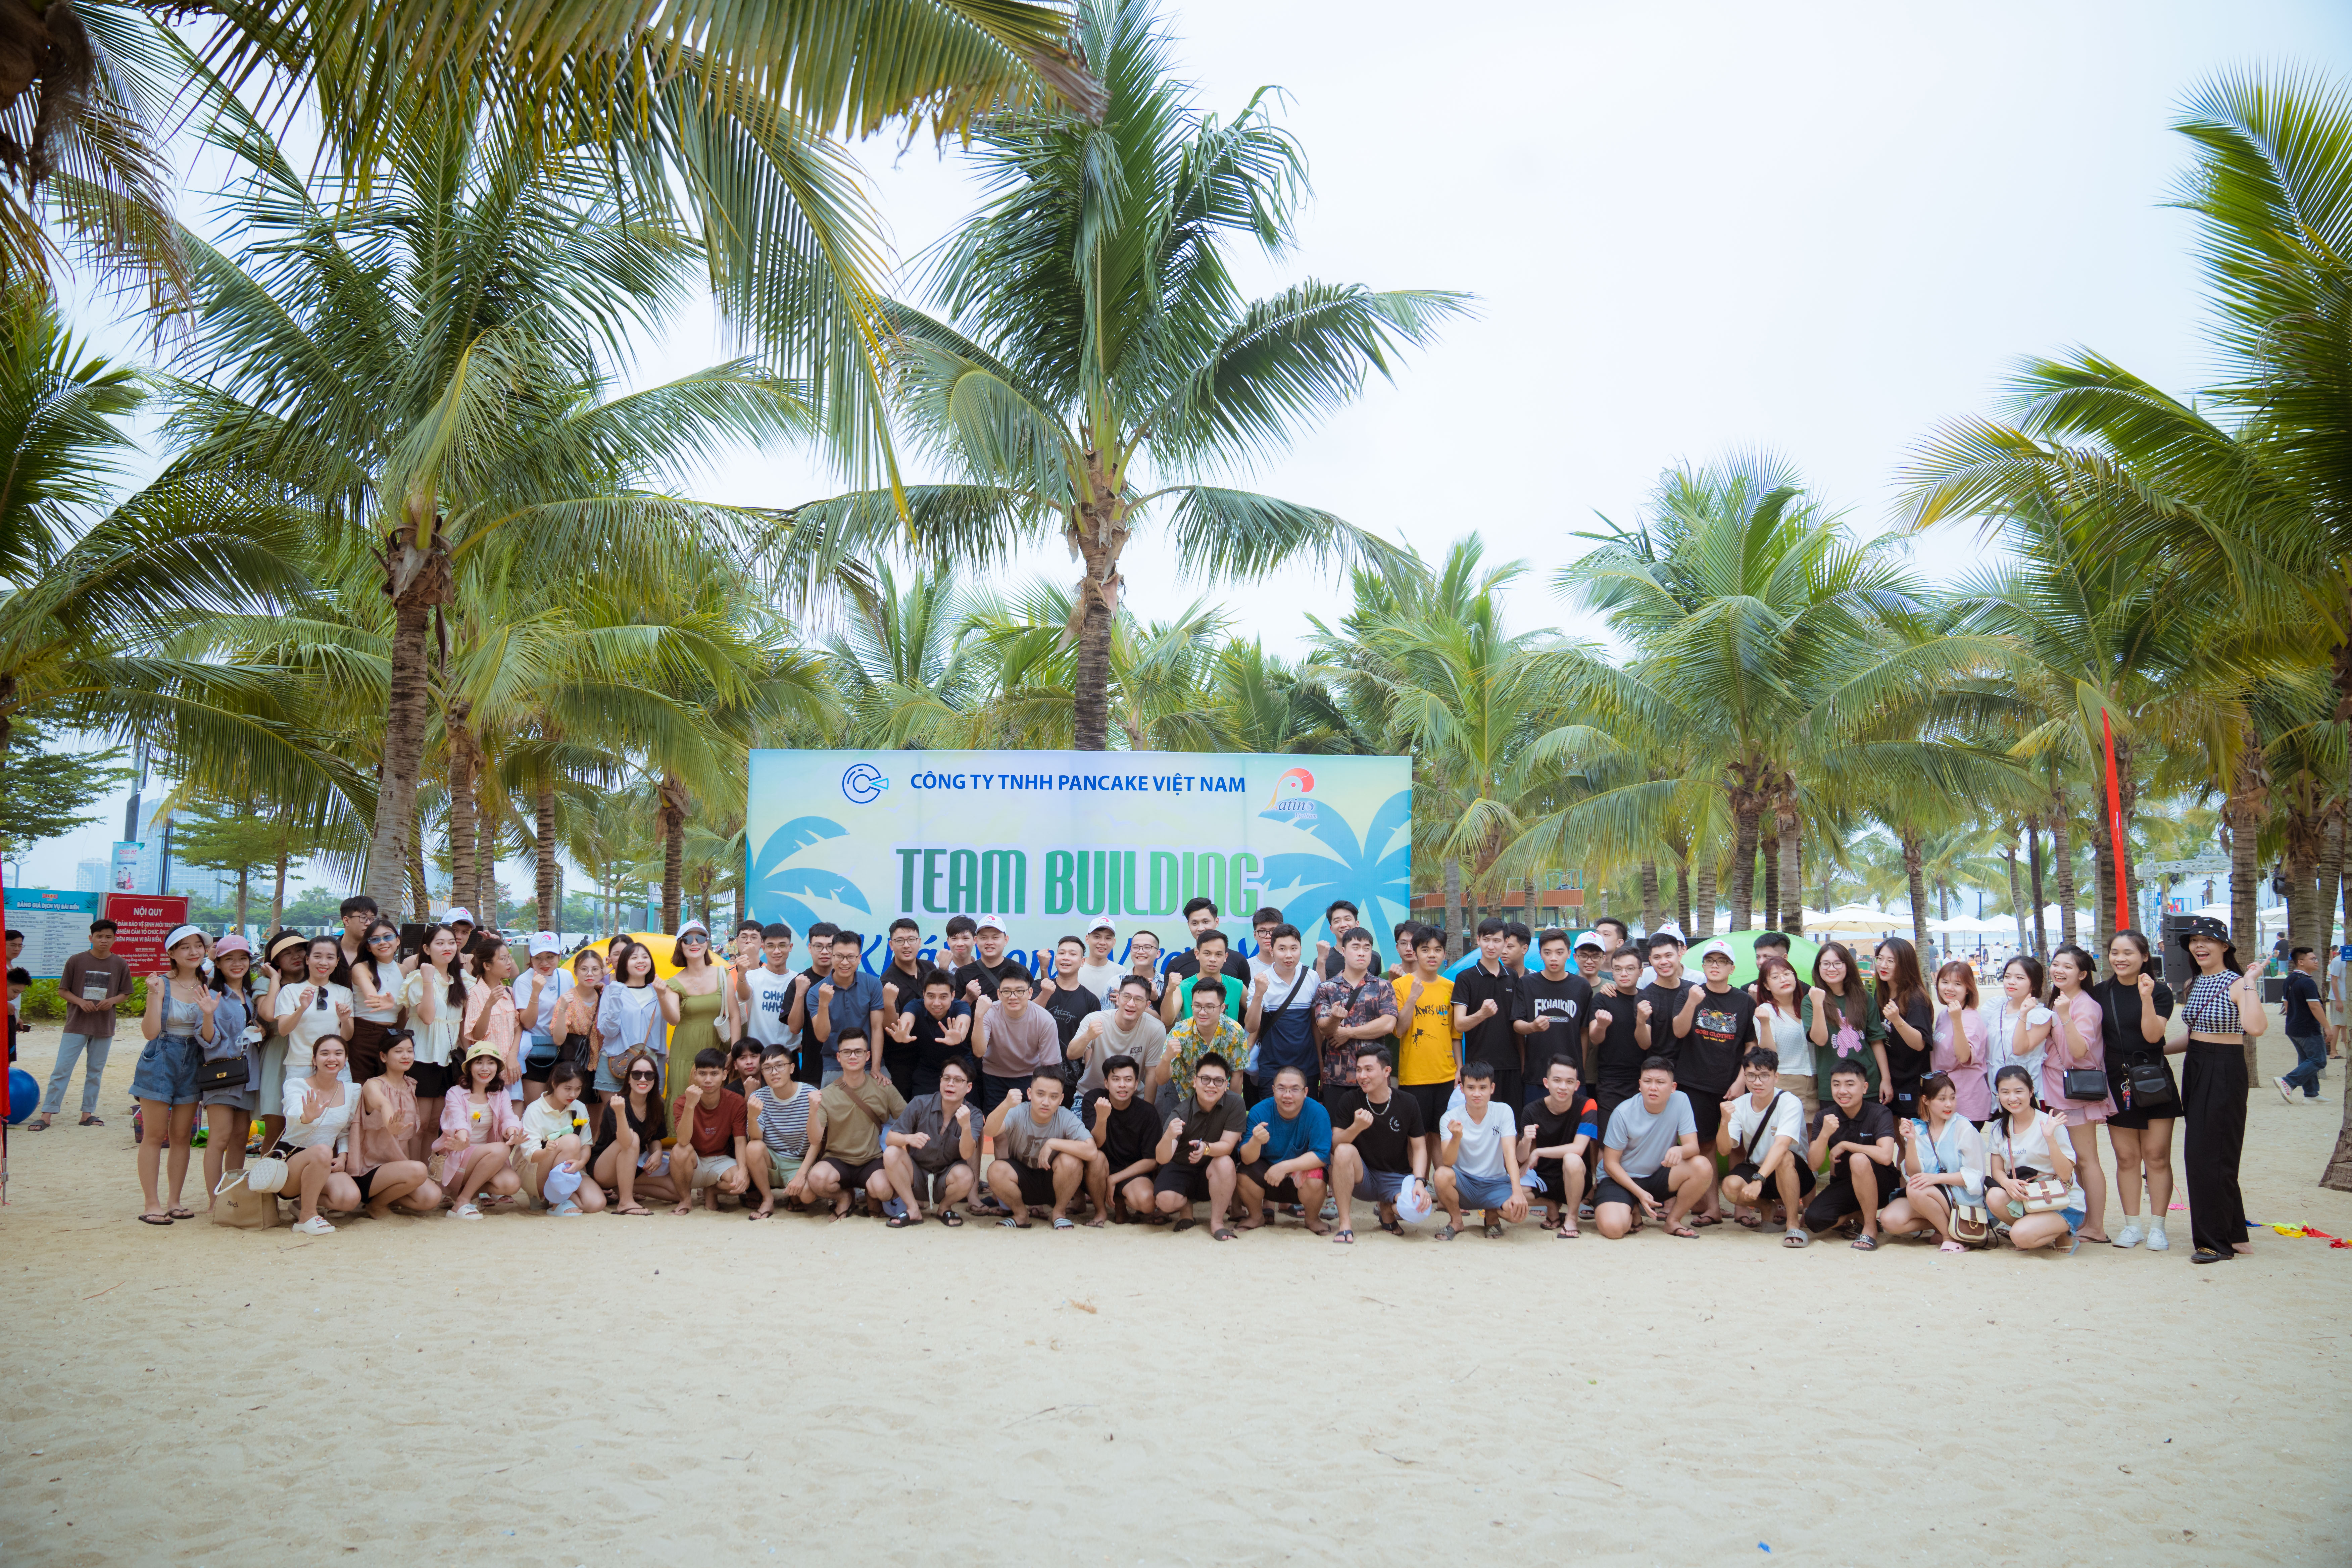
\includegraphics[width=14cm,height=9.2cm]{Images/pancake/pancake_travel.jpg}
  \caption[Hình ảnh du lịch của công ty]{\bfseries \fontsize{12pt}{0pt}
  \selectfont Hình ảnh du lịch của công ty}
  \label{ttlk} %đặt tên cho ảnh
\end{figure}


\subsection{Kết luận chương}
Trong chương này, em đã giới thiệu về công ty và trình bày khái quát về các sản phẩm và hoạt động ngoại khoá của công ty
em được trải nghiệm trong thời gian thực tập.

\newpage
